%lecture 1

\begin{theorem}[L1.1]{Weierstrass.}
    Let $f: \Omega \rightarrow \mathbb{R}$ be a continuous function defined on a nonempty and compact (i.e., closed and bounded) set $\Omega$. Then, there exists a minimizer $x^* \in \Omega$ of $f$ on $\Omega$, that is,
    \vspace{-4pt}\\
    $$
    f\left(x^*\right) \leq f(x) \quad \text { for all } x \in \Omega
    $$
    \vspace{-7pt}
\end{theorem}

\begin{theorem}[L1.2]{Weierstrass for Compact Sublevel Sets.}
    Let $f$ be a continuous function defined on a set $S$. If $f$ has a nonempty and compact sublevel set, that is, there exists $\alpha \in \mathbb{R}$ such that
    \vspace{-4pt}\\
    $$
    \{x \in S: f(x) \leq \alpha\}
    $$
    \vspace{-4pt}\\
    is nonempty, bounded, and closed, then $f$ has a minimizing point in $S$.
\end{theorem}


% lecture 2

\begin{definition}[L2.1]{Star-convexity at $x$.} 
    A set $\Omega \subseteq \mathbb{R}^n$ is said to be star-convex at a point $x \in \Omega$ if, for all $y \in \Omega$, the entire segment from $x$ to $y$ is contained in $\Omega$. In symbols, if
    \vspace{-4pt}\\
    $$
    x+t \cdot(y-x) \in \Omega \quad \forall t \in[0,1]
    $$
    \vspace{-7pt}\\
    (Note that the condition is equivalent to \\
    "$t \cdot y+(1-t) \cdot x \in \Omega$ $\forall$ $y \in \Omega$, $t \in$ $[0,1]$ ", or also \\
    "$t \cdot x+(1-t) \cdot y \in \Omega$ $\forall$ $y \in \Omega$, $t \in[0,1]$ ".)
\end{definition}

\begin{definition}[L2.2]{Convex set.} 
    A set $\Omega$ is convex if it is star-convex at all of its points $x \in$ $\Omega$. In other words, $\Omega$ is convex if all segments formed between any two points $x, y \in \Omega$ are entirely contained in $\Omega$. In symbols, if
    \vspace{-4pt}\\
    $$
    t \cdot x+(1-t) \cdot y \in \Omega \quad \forall x, y \in \Omega \text { and } t \in[0,1] .
    $$
    \vspace{-4pt}
\end{definition}

\begin{theorem}[L2.1]{First-order necessary condition for a convex feasible set}
    Let $\Omega \subseteq \mathbb{R}^n$ be convex and $f: \mathbb{R}^n \rightarrow \mathbb{R}$ be a differentiable function. For a point $x \in \Omega$ to be a minimizer of $f$ over $\Omega$ it is necessary that
    \vspace{-4pt}\\
    $$
    \langle\nabla f(x), y-x\rangle \geq 0 \quad \forall y \in \Omega
    $$
    \vspace{-4pt}
\end{theorem}

\begin{definition}[L2.3]{Normal cone.}
    Let $\Omega \subseteq \mathbb{R}^n$ be convex, and let $x \in \Omega$. The normal cone to $\Omega$ at $x$, denoted $\mathcal{N}_{\Omega}(x)$, is defined as the set
    \vspace{-4pt}\\
    {\footnotesize$$
    \mathcal{N}_{\Omega}(x):=\left\{d \in \mathbb{R}^n:\langle d, y-x\rangle \leq 0 \quad \forall y \in \Omega\right\} .
    $$}
    \vspace{-4pt}\\
    With this definition, the first-order necessary optimality condition for $x$, given in Th L2.1, can be equivalently written as
    \vspace{-4pt}\\
    $$
    -\nabla f(x) \in \mathcal{N}_{\Omega}(x)
    $$
    \vspace{-4pt}\\
    Normal cone at interior $N_{\Omega}(x) = \{0\}$ (consider $y=x+\delta d$ and realize $\langle d, y-x\rangle > 0$).
\end{definition}

\begin{theorem}[L2.2]{Normal cone to a hyperplane.}
    Consider a hyperplane
    \vspace{-4pt}\\
    $$
    \Omega := \{y \in \mathbb{R}^n : \langle a, y \rangle = b\},
    $$
    \vspace{-7pt}\\
    where $a \in \mathbb{R}^n,\, a \neq 0,$
    and a point $x \in \Omega$. The normal cone at $x$ is given by
    \vspace{-4pt}\\
    $$
    \mathcal{N}_{\Omega}(x) = \operatorname{span}\{a\} = \{\lambda a : \lambda \in \mathbb{R}\}.
    $$
    \vspace{-7pt}\\
    (consider $y \in \operatorname{span}\{a\}$ and $z=(y-x) = k\cdot a \notin \operatorname{span}\{a\}$)
    Similarly, for affine subspaces $\Omega = \{y \in \mathbb{R}^n : Ay = b\}$, the normal cone is $\mathcal{N}_{\Omega}(x) = \operatorname{colspan}\{A^\top\} = \{A^\top \lambda : \lambda \in \mathbb{R}^n\}$.
    (project $x+z$ onto $\Omega$ and $\operatorname{colspan}(A^\top)$)
\end{theorem}

% lecture 3

\begin{theorem}[L3.1,L5.3]{Normal cone to the intersection of m halfspaces.}
    Let $\Omega \subseteq \mathbb{R}^n$ be given as the intersection of $m$ linear inequalities $\langle a_j, x\rangle \leq b_j$. Then, the normal cone at any point $x \in \Omega$ is obtained by taking nonnegative combinations of all those $a_j$ 's for which $\langle a_j, x\rangle=b_j$. 
    \vspace{-4pt}\\
    $$
    \mathcal{N}_{\Omega}(x)=\left\{\sum_{j \in I(x)} \lambda_j \cdot a_j: \lambda_j \in \mathbb{R}_{\geq 0}\right\},
    $$ 
    \vspace{-4pt}\\
    where $I(x)=\left\{j \in\{1, \ldots, m\}:\langle a_j, x\rangle=b_j\right\}$.\\
    The constraints $j$ in $I(x)$ are often called the "active constraints" at $x \in \Omega$.
    Alternatively in vectorial form let $Ax \leq b$, then with $A\in \mathbb{R}^{m \times n}, b \in \mathbb{R}^m$:
    \vspace{-4pt}\\
    {\footnotesize$$
    \begin{aligned}
        \mathcal{N}_{\Omega}(x) &= \left\{\sum_{j=1}^{m} \lambda_j a_j : \sum_{j=1}^{m} \lambda_j  \left(b_j - \langle a_j, x \rangle \right) = 0 ;\text{ } \lambda_j \geq 0 \right\}\\
        &= \left\{A^{\top} \lambda: \lambda^{\top}(b-A x)=0, \lambda \in \mathbb{R}_{\geq 0}^m\right\},
    \end{aligned}
    $$
    \vspace{-10pt}\\
    $$
    A=\left(\begin{array}{c}
        -a_1^{\top}- \\
        \vdots \\
        -a_m^{\top}-
        \end{array}\right),
    $$}
    rewriting the condition $j \in I(x)$ (via \textbf{complementary slackness}).
\end{theorem}

\begin{remark}[L3.3]{Primal and Dual}
    Consider the linear program
    \vspace{-5pt}\\
    \begin{equation}
        \begin{array}{cl}
            \max _x & c^{\top} x \\
            \text { s.t. } & A x \leq b \\ 
            & x \in \mathbb{R}^n,
        \end{array}\tag{P}
    \end{equation}
    \vspace{-5pt}\\
    \begin{equation}
        \begin{array}{cl}
            \min _\lambda & g(\lambda):=b^{\top} \lambda \\
            \text { s.t. } & A^{\top} \lambda=c \\
            & \lambda \geq 0
        \end{array}\tag{D}
    \end{equation}
    \vspace{-5pt}
\end{remark}

\begin{theorem}[L3.2]{Strong linear programming duality.}
    If (P) admits an optimal solution $x^*$, then (D) admits an optimal solution $\lambda^*$, such that:
    \begin{itemize}[leftmargin=*]
        \item the values of the two problems coincide: $c^{\top} x^*=b^{\top} \lambda^*$, and
        \item $\lambda^*$ satisfies the complementary slackness condition $(\lambda^*)^{\top}(b-A x^*)=0$.
    \end{itemize} 
\end{theorem}

% lecture 4

% \begin{definition}[L4.1]{Convex function.}\hfill
%     \vspace{2pt}\\
%     Let $\Omega \subseteq \mathbb{R}^n$ be convex.
%     A function $f: \Omega \rightarrow \mathbb{R}$ is convex if, for any two points $x, y \in \Omega$ and $t \in[0,1]$,
%     \vspace{-4pt}\\
%     $$
%     \begin{aligned}
%         f((1-t) \cdot x+t \cdot y) &\leq (1-t) \cdot f(x)+t \cdot f(y)\\
%         f(x + t(y-x)) &\leq f(x) + t(f(y) - f(x))
%     \end{aligned}
%     $$
%     \vspace{-4pt}
%     % \end{minipage}\hfill
%     % \begin{minipage}[c]{0.32\textwidth}
%     %     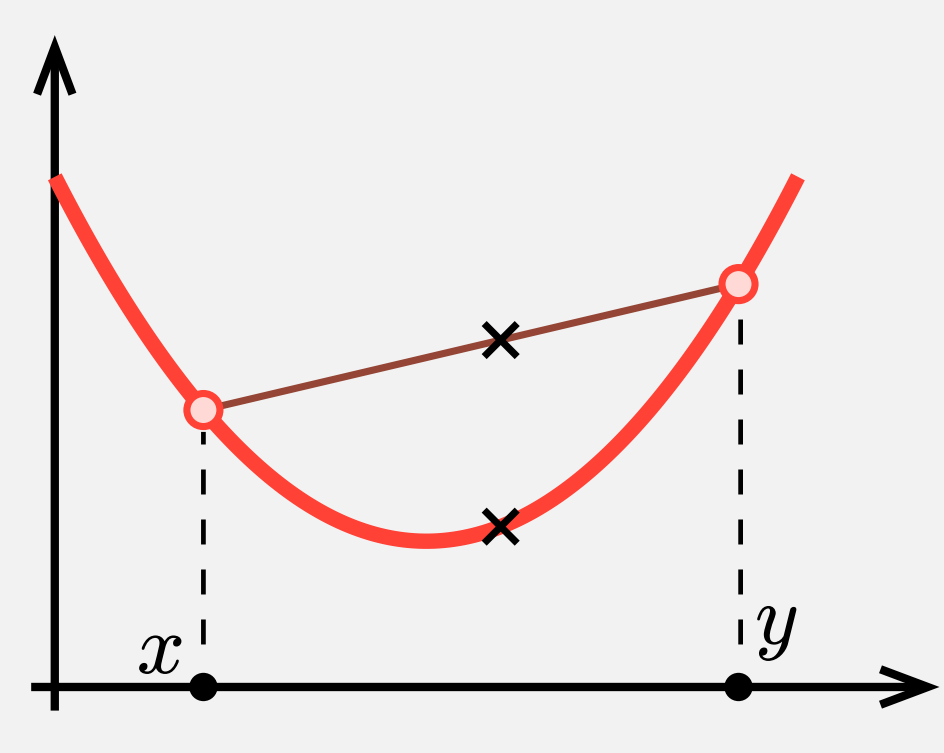
\includegraphics[width=\linewidth]{figures/convex_function.png}
%     % \end{minipage}  
% \end{definition}

% \begin{theorem}[L4.1]{Bounding by linearization.}
%     Let $f: \Omega \rightarrow \mathbb{R}$ be a convex and differentiable function defined on a convex domain $\Omega$. Then, at all $x \in \Omega$,
%     \vspace{-4pt}\\
%     $$
%     f(y) \geq \underbrace{f(x)+\langle\nabla f(x), y-x\rangle}_{\text {linearization of } f \text { around } x} \quad \forall y \in \Omega .
%     $$
%     \vspace{-4pt}\\
%     (definition of convexity, divide by $t$ and take limit)
% \end{theorem}

\begin{theorem}[L4.2]{Sufficiency of first-order optimality condition.}
    Let $\Omega \subseteq \mathbb{R}^n$ be convex and $f: \Omega \rightarrow \mathbb{R}$ be a convex differentiable function. Then,
    \vspace{-4pt}\\
    \begin{equation*}
        -\nabla f(x) \in \mathcal{N}_{\Omega}(x) \text{ } \Leftrightarrow \text{ } \text{$x$ is minimizer of $f$ on $\Omega$}
    \end{equation*}
    \vspace{-7pt}
\end{theorem}

\begin{theorem}[L4.3]{Equivalent definitions of convexity.}
    Let $\Omega \subseteq \mathbb{R}^n$ be a convex set, and $f: \Omega \rightarrow \mathbb{R}$ be a function. The following are equivalent definitions of convexity for $f$ :
    \begin{enumerate}[leftmargin=*]
        \item for all $x, y \in \Omega, t \in[0,1]$:
        \vspace{-4pt}\\
        $$
            \begin{aligned}
                f((1-t) \cdot x+t \cdot y) &\leq (1-t) \cdot f(x)+t \cdot f(y)\\
                f(x + t(y-x)) &\leq f(x) + t(f(y) - f(x))
            \end{aligned}
        $$
        \vspace{-4pt}
        \item $f(y) \geq f(x)+\langle\nabla f(x), y-x\rangle$ for all $x, y \in \Omega$ [If $f$ is differentiable]
        \item $\langle\nabla f(y)-\nabla f(x), y-x\rangle \geq 0$ for all $x, y \in \Omega$ [If $f$ is differentiable]
        \item $\nabla^2 f(x) \succeq 0$ for all $x \in \Omega$ [If $f$ is twice differentiable and $\Omega$ is open]
    \end{enumerate}
    $(1) \Rightarrow (2)$ \textbf{Bounding by linearization}: Divide by $t$ and take limit.\\
    $(2) \Rightarrow (1)$ Sum linearization bounds (multiplied by $t$ and $1-t$ accordingly) centered in point $z := t \cdot x + (1-t) \cdot y$ and look in directions $x-z$ and $y-z$.\\
    $(2) \Rightarrow (3)$ Write condition $(2)$ for $(x,y)$ and $(y,x)$ and take sum.\\
    $(3) \Rightarrow (4)$ Consider $x_t:=x+t \cdot (y-x)$ and plug into $(3)$ for $y$. Divide by $t^2$, take limit.\\
    $(4) \Rightarrow (3)$ Use $0\leq \langle y-x, \nabla^2 f(x + \tau (y-x))\cdot (y-x)\rangle$ and integrate $\tau\in[0,1]$.\\
    $(3) \Rightarrow (2)$ Define $x_t$ as above, integrate $t \cdot \langle \nabla f(x_t) - \nabla f(x), y-x\rangle$ for $t\in[0,1]$.
\end{theorem}

\begin{theorem}[L4.4]{Operations preserving convexity.}
    \begin{itemize}[leftmargin=*]
        \item Multiplication of a convex function $f(x)$ by a nonnegative scalar $c \geq 0$;
        \item Addition of two convex functions $f(x), g(x)$;
        \item Pointwise supremum of a collection $J$ of convex functions $\left\{f_j(x): j \in J\right\}$ :
        \vspace{-4pt}\\
        $$
        f_{\max }(x):=\max _{j \in J} f_j(x) ;
        $$
        \vspace{-10pt}
        \item Pre-composition $f(A x+b)$ of a convex function $f$ with an affine function $A x+b$.
        \item Post-composition $g(f(x))$ of a convex function with an increasing convex function $g$;
        \item Infimal convolution $f \iconv g$ of two convex functions $f, g: \mathbb{R}^n \rightarrow \mathbb{R}$, defined as
        \vspace{-4pt}\\
        $$
        \inf \left\{f(y)+g(x-y): y \in \mathbb{R}^n\right\}
        $$
        \vspace{-4pt}
    \end{itemize}

\end{theorem}

\begin{definition}[L4.2]{Strict and strong convexity.}
    Let $\Omega \subseteq \mathbb{R}^n$ be convex.
    \begin{itemize}[leftmargin=*]
        \item A function $f: \Omega \rightarrow \mathbb{R}$ is strictly convex if, for any two distinct points $x, y \in \Omega$ and $t \in(0,1)$,
        \vspace{-4pt}\\
        $$
        f((1-t) \cdot x+t \cdot y)<(1-t) \cdot f(x)+t \cdot f(y)
        $$
        \vspace{-10pt}
        \item For $f$ twice differentiable and $\Omega$ open, $\nabla^2 f(x) \succ 0 \text{ } \forall x \in \Omega$  is sufficient for strict convexity.
        \item A function $f: \Omega \rightarrow \mathbb{R}$ is strongly convex with modulus $\mu>0$ if the function
        \vspace{-5pt}\\
        $$
        f(x)-\frac{\mu}{2}\|x\|_2^2
        $$
        \vspace{-5pt}\\
        is convex.
        Note that strong convexity implies strict convexity, and strict convexity implies convexity. Neither of the reverse implications holds.
        \item For $f$ twice differentiable and $\Omega$ open, strong convexity is equivalent to $\nabla^2 f(x) \succeq \mu I \text{ } \forall x \in \Omega$. 
        \item For $f$ twice differentiable and $\Omega$ open, strong convexity is equivalent to $f(y) \geq f(x) + \langle \nabla f(x), y-x\rangle + \frac{\mu}{2}\|y-x\|_2^2 \text{ } \forall x,y\in\Omega$.
    \end{itemize}
\end{definition}

\begin{theorem}[L4.5]{Strict convexity and uniqueness of minimizer.}
    Let $\Omega \subseteq \mathbb{R}^n$ be convex, and $f: \Omega \rightarrow \mathbb{R}$ be a strictly convex function. Then, $f$ has at most one minimizer.
    (Set $f(x)=f(y)=f^\star$ and use strict convexity.)\\
    \textbf{Corollary (Projection onto convex set):} Since the function $\|x-y\|_2^2$ is strongly convex, and hence strictly convex, it follows that any projection onto a convex set $\Omega$, if it exists, is unique.
\end{theorem}

% lecture 5

\begin{theorem}[L5.1]{Separation}
    Let $\Omega \subseteq \mathbb{R}^n$ be a nonempty, closed, and convex set, and let $y \in \mathbb{R}^n$ be a point. If $y \notin \Omega$, then there exist $u \in \mathbb{R}^n, v \in \mathbb{R}$ such that
    \vspace{-4pt}\\
    $$
    \langle u, y\rangle<v, \quad \text { and } \quad\langle u, x\rangle \geq v \quad \forall x \in \Omega .
    $$
    \vspace{-4pt}\\
    (Let $x^\star$ be projection of $y$ on $\Omega$, then $u = x^\star - y$ and $v = \langle u, x^\star\rangle$. \textbf{Note:} For strict inequality let $v^\prime:=\frac{1}{2}(\langle u, x^\prime \rangle + \langle u, y \rangle)$)\\
\end{theorem}

\begin{definition}[L5.1]{Cone}
    A set $S$ is a cone if, for any $x \in S$ and $\lambda \in \mathbb{R}_{\geq 0}$, the point $\lambda \cdot x \in S$.
\end{definition}

\begin{theorem}[L5.2]{Separation of a point from a cone.}
    Let $S \subseteq \mathbb{R}^n$ be a nonempty closed convex cone, and $y \notin S$ be a point in $\mathbb{R}^n$. Then, there exists a hyperplane passing through the origin that separates $y$ from $S$; formally, there exists $u \in \mathbb{R}^n$ such that
    \vspace{-4pt}\\
    $$
    \langle u, y\rangle<0 \quad \text { and } \quad\langle u, x\rangle \geq 0 \quad \forall x \in S
    $$
    \vspace{-8pt}
\end{theorem}

\begin{definition}[L5.2]{(Strong) separation oracle}
    Let $\Omega \subseteq \mathbb{R}^n$ be convex and closed. A strong separation oracle for $\Omega$ is an algorithm that, given any point $y \in \mathbb{R}^n$, correctly outputs one of the following:
    \begin{itemize}[leftmargin=*]
        \item " $y \in \Omega$ ", or
        \item $(y \notin \Omega, u)$ ", where the vector $u \in \mathbb{R}^n$ is such that
        \vspace{-5pt}\\
        $$
        \langle u, y\rangle<\langle u, x\rangle \quad \forall x \in \Omega
        $$
        \vspace{-8pt}
    \end{itemize}
    \textbf{Note}: separation oracle for convex polytope: If $Ay \leq b$ return " $y \in \Omega$ ", otherwise return $(y \notin \Omega, -a)$, where $a$ is a violated constraint.
\end{definition}

\begin{remark}[L5.4]{Ellipsoid method.}
    at each iteration, start with a search ellipsoid $\varepsilon_1$, feasible set $\Omega_1 = \Omega$, and the center of the ellipsoid $c_t$.
    \begin{itemize}[leftmargin=*]
        \item if $c_t \notin \Omega_t$, then $\varepsilon_{t+1}$ contains the intersection between $\varepsilon_t$ and the halfspace containing $\Omega_t$ returned by the separation oracle
        \item if $c_t \in \Omega_t$, let $H_t = \{x \in \mathbb{R}^n : \langle \nabla f(c_t), x - c_t\rangle \leq 0\}$, $\Omega_{t+1} := \Omega_t \cap H_t$, and $\varepsilon_{t+1} := \varepsilon_t \cap H_t$. (to make the search space contain only points x such that $f(x) \leq f(c_t)$ by Th.L4.3)
    \end{itemize}
\end{remark}

\begin{theorem}[L5.4]{Ellipsoid method for convex optimization.}
    Theorem L5.4. Let $R$ and $r$ be as above, and let the range of the function $f$ on $\Omega$ be bounded by $[-B, B]$. Then, the ellipsoid method described above run for $T \geq$ $2 n^2 \log (R / r)$ steps either correctly reports that $\Omega=\emptyset$, or produces a point $x^{\star}$ such that
    \vspace{-4pt}\\
    {\footnotesize$$
    f\left(x^{\star}\right) \leq f(x)+\frac{2 B R}{r} \exp \left(-\frac{T}{2 n(n+1)}\right) \quad \forall x \in \Omega .
    $$}
    \vspace{-4pt}
\end{theorem}

% lecture 6

\begin{theorem}[L6.1]{Farkas lemma.}
    Let $A x \leq b$ be a system of inequalities where $A \in \mathbb{R}^{m \times n}$. Then, exactly one of the following options is true:
    \begin{itemize}[leftmargin=*]
        \item either $A x \leq b$ has a solution; or
        \item there exists a vector $y \geq 0$ such that $A^{\top} y=0$ and $b^{\top} y<0$.
    \end{itemize}
    \vspace{-4pt}
    (Let $\Omega = \{Ax+s : x \in \mathbb{R}^n, s \in \mathbb{R}^m_{\geq0}\}$. If $b\in\Omega$, $Ax\leq b$ has a solution. Else, apply separation, first set $s=x=0$: $v\leq 0$, $\langle u,b \rangle < 0$, then $s=0$: $\langle A^\top u, x \rangle \geq v$, finally set $x=0$, $s=ke_i\geq0$)\\
\end{theorem}

% lecture 7

\begin{remark}[L7.1]{Optimization Problem with differentiable functional constraints.}
    We consider an optimization problem with constraint set defined as the intersection of differentiable functional constraints: 
    \begin{equation}
        \begin{array}{ll}
            \min _x & f(x) \\
            \text { s.t. } & h_i(x)=0 \quad i \in\{1, \ldots, r\} \\
            & g_j(x) \leq 0 \quad j \in\{1, \ldots, s\}.
        \end{array} \tag{1}
    \end{equation}
    \vspace{-7pt}\\
    Note, that in L8, we refer to $(P)$ as the same problem with $f$ convex, $g_j$ convex, and $h_i$ affine.
\end{remark}


\begin{theorem}[L7.1]{Normal cone to the intersection of linear inequalities. (rewriting L3.1,L5.3)}
    Let $\Omega \subseteq \mathbb{R}^n$ be defined as the intersection of $m$ linear inequalities
    \vspace{-4pt}\\
    {\footnotesize$$
    \Omega:=\left\{x \in \mathbb{R}^n: \begin{array}{ll}
        a_i^{\top} x=b_i & \forall i=1, \ldots, r \\
        c_j^{\top} x \leq d_j & \forall j=1, \ldots, s
        \end{array}\right\}
    $$}
    \vspace{-4pt}\\
    Given a point $x \in \Omega$, define the index set of the "active" inequality constraints
    \vspace{-4pt}\\
    $$
    I(x):=\left\{j \in\{1, \ldots, s\}: c_j^{\top} x=d_j\right\} .
    $$
    \vspace{-4pt}\\
    Then, the normal cone at any $x \in \Omega$ is given by $\mathcal{N}_{\Omega}(x)={}$
    \vspace{-4pt}\\
    {\footnotesize
    $$
    \begin{aligned}
    =&\left\{\sum_{i=1}^r \mu_i a_i+\sum_{j \in I(x)} \lambda_j c_j: \mu_i \in \mathbb{R}, \lambda_j \in \mathbb{R}_{\geq 0}\right\} \\
    =&\left\{\sum_{i=1}^r \mu_i a_i+\sum_{j=1}^s \lambda_j c_j: \mu_i \in \mathbb{R}, \lambda_j \in \mathbb{R}_{\geq 0}\right.,\\
    &\quad\left.\lambda_j\left(d_j-c_j^{\top} x\right)=0 \text{ } \forall j=1, \ldots, s\right\},\\
    \end{aligned}
    $$
    }
    \vspace{-4pt}\\
    where the second equality simply rewrites the condition $j \in I(x)$ via complementary slackness (see L3.1).
\end{theorem}

\newpage


\begin{definition}[L7.1]{KKT conditions.}
    Consider a nonlinear optimization problem with differentiable objective function and functional constraints, in the form given in (1), and let $x$ be a point in the feasible set (``Primal Feasibility''). The KKT conditions at $x$ are given by
    \begin{itemize}[leftmargin=*]
        \item \textbf{Stationarity}:\\
        $-\nabla f(x)=\sum_{i=1}^r \mu_i \nabla h_i(x)+\sum_{j=1}^s \lambda_j \nabla g_j(x)$
        \vspace{-2pt}\\
        \item \textbf{Dual feasibility}:\\
        $\mu_i \in \mathbb{R}, \quad \lambda_j \geq 0 \quad \forall i=1, \ldots, r, \quad j=1, \ldots, s .$
        \vspace{-2pt}\\
        \item \textbf{Complementary slackness}:\\
        $\lambda_j \cdot g_j(x) =0 \forall j=1, \ldots, s .$
    \end{itemize}
    (Note: Example of failure of KKT: $f(x) = x, g(x) = x^2$)
\end{definition}



\begin{theorem}[L7.2]{Concave and linear constraints.}
    Let $x \in \Omega \subseteq \mathbb{R}^n$ be a minimizer of (1). If
    \begin{itemize}[leftmargin=*]
        \item the binding inequality constraints $\left\{g_j\right\}_{j \in I(x)}$ are concave differentiable functions in a convex neighborhood of $x$; and
        \item the equality constraints $\left\{h_i\right\}_{i=1}^r$ are affine functions on $\mathbb{R}^n$, 
    \end{itemize}
    then the KKT conditions hold at $x$ (Necessity of KKT conditions).
\end{theorem}


\begin{theorem}[L7.3]{Linear independence of gradients.}
    Let $x \in \Omega \subseteq \mathbb{R}^n$ be a minimizer of (1). If all functions $h_i, g_j$ are continuously differentiable and the multiset of gradients at $x$ of all active constraints
    \vspace{-4pt}\\
    $$
    \left\{\nabla h_i(x): i=1, \ldots, r\right\} \cup\left\{\nabla g_j(x): j \in I(x)\right\}
    $$
    \vspace{-4pt}\\
    is linearly independent, then the KKT conditions hold at $x$.
\end{theorem}

\begin{theorem}[L7.4]{Slater's condition.}
    Let $x \in \Omega \subseteq \mathbb{R}^n$ be a minimizer of (1). If
    \begin{itemize}[leftmargin=*]
        \item the binding inequality constraints $\left\{g_j\right\}_{j \in I(x)}$ are convex differentiable functions; and 
        \item the equality constraints $\left\{h_i\right\}_{i=1}^r$ are affine functions; and
        \item there exists a feasible point $x_0$ that is strictly feasible for the binding inequality constraints, that is,
        \vspace{-4pt}\\
        $$
        g_j\left(x_0\right)<0 \quad \forall j \in I(x)
        $$
        \vspace{-4pt}\\
        then the KKT conditions hold at $x$.
    \end{itemize}
\end{theorem}

\begin{theorem}[L7.5]{Necessity and sufficiency of KKT conditions.}
    If $f$ is convex and the constraints satisfy Slater's condition, then the KKT conditions are both necessary and sufficient for optimality.
    (Note: Proof by checking KKT conditions, then formulate Lagrangian, and conclude with $f(x) \geq L(x) = L(x^\star) = f(x^\star)$)
\end{theorem}

%lecture 8

\begin{remark}[L8.1]{Equivalence at Optimality}
    The following statements are equivalent:
    \begin{itemize}[leftmargin=*]
        \item The point $x^\star\in \Omega$ is optimal for (P).
        \item the point $x^\star$ admits $\mu^\star$, $\lambda^\star$ such that the KKT conditions hold.
        \item there exist $\mu^\star$, $\lambda^\star$ such that $x^\star$ is minimizer of Lagrangian.
    \end{itemize}
    Note: the Lagrangian of (P) is:
    \vspace{-4pt}\\
    $$
    \mathcal{L}(x ; \lambda, \mu)=f(x)+\sum_{j=1}^{r} \lambda_{j} g_{j}(x)+\sum_{i=1}^{s} \mu_{i} h_{i}(x), \quad \lambda \geq 0
    $$
    \vspace{-4pt}
\end{remark}

\begin{theorem}[L8.1]{Existence of finite penalization coefficients.}
    If the constrained problem (P) has a minimizer $x^* \in \Omega$ and attains optimal value value $(P)$, there exist concrete penalization coefficients $\left(\lambda^*, \mu^*\right) \in \mathbb{R}_{\geq 0}^r \times \mathbb{R}^s$ such that
    \vspace{-4pt}\\
    \begin{enumerate}[leftmargin=*]
        \item $x^*$ is a minimizer of $x \mapsto \mathcal{L}\left(x ; \lambda^*, \mu^*\right)$ over $\mathbb{R}^n$; and
        \item the value of $\min _{x \in \mathbb{R}^n} \mathcal{L}\left(x ; \lambda^*, \mu^*\right)$ is exactly equal to value $(P)$.
    \end{enumerate}
    Conversely, if there is a triple $\left(x^* ; \lambda^*, \mu^*\right) \in \mathbb{R}^n \times\left(\mathbb{R}_{\geq 0}^r \times \mathbb{R}^s\right)$ such that $x^*$ is a minimizer of $\mathcal{L}\left(x ; \lambda^*, \mu^*\right)$, and it satisfies $x^* \in \Omega, \lambda_j^* g_j\left(x^*\right)=0$ for all $j=1, \ldots, r$, then $x^*$ is also an optimal solution of $(\mathrm{P})$.
\end{theorem}

\begin{theorem}[L8.2]{Weak duality.}
    For any choice of penalization coefficients $\lambda \in \mathbb{R}_{\geq 0}^r, \mu \in \mathbb{R}^s$,
    \vspace{-4pt}\\
    $$
    \inf _x \mathcal{L}(x ; \lambda, \mu) \leq f(\tilde{x}) \quad \forall \tilde{x} \in \Omega
    $$
    \vspace{-4pt}\\
    In fact, the inequality holds for any minimization problem with functional constraints -- that is, even ignoring the requirement that $g_j$ is convex, that $h_i$ is affine, and any constraint qualification.

    As a direct consequence, if (P) admits an optimal solution, then
    \vspace{-4pt}\\
    $$
    \inf _x \mathcal{L}(x ; \lambda, \mu) \leq \sup_{\lambda \geq 0, \mu}\inf _x \mathcal{L}(x ; \lambda, \mu) \leq \text { value }(P)
    $$
    \vspace{-4pt}\\
    \textbf{Corollary (Strong Duality)}:\\
    Corollary L8.1 (Strong duality). If (P) admits a minimizer, the optimization problem
    \vspace{-4pt}\\
    $$
    (D):= \begin{cases}\max _{\mu, \lambda} & \inf _{x \in \mathbb{R}^n} \mathcal{L}(x ; \lambda, \mu) \\ \text { s.t. } & \lambda \in \mathbb{R}_{\geq 0}^r \\ & \mu \in \mathbb{R}^s\end{cases}
    $$
    \vspace{-4pt}\\
    admits an optimal solution $\lambda^*, \mu^*$, and matches the value of the original problem (P).
\end{theorem}

\begin{remark}[L8.3]{Strong Duality statement.}
    If (P) has an optimal solution, then
    \vspace{-4pt}\\
    \begin{equation*}
        \begin{aligned}
            \operatorname{value}(D) &= \max _{\lambda \in \mathbb{R}_{\geq 0}^r, \mu \in \mathbb{R}^s} \inf _{x \in \mathbb{R}^n} \mathcal{L}(x ; \lambda, \mu) = \\
            =\operatorname{value}(P) &= {\min _{x \in \mathbb{R}^n} \sup _{\lambda \in \mathbb{R}_{\geq 0}^r, \mu \in \mathbb{R}_{ }^s} \mathcal{L}(x ; \lambda, \mu) .}
        \end{aligned}
    \end{equation*}
    \vspace{-4pt}
\end{remark}

% lecture 9

\begin{remark}[L9.1]{Conic Optimization Problem.}
    Feasible set is intersection between affine subspace and nonempty closed convex cone $\mathcal{K}$:
    \vspace{-4pt}\\
    \begin{equation}
        \begin{array}{cl}
        \min _x & f(x) \\
        \text { s.t. } & A x=b \\
        & x \in \mathcal{K}
        \end{array}\tag{2}
    \end{equation}
    \vspace{-4pt}
\end{remark}


\begin{definition}[L9.1]{Lorentz (ice-cream) cone.}
    In second-order conic programs (SOCPs):
    \vspace{-4pt}\\
    $$
    \mathcal{L}^n:=\left\{(x, z) \in \mathbb{R}^{n-1} \times \mathbb{R}: z \geq\|x\|_2\right\}
    $$
    \vspace{-4pt}
\end{definition}

\begin{definition}[L9.2]{Semidefinite cone.}
    The semidefinite cone $\mathcal{S}^n$ is the set of positive semidefinite $n \times n$ matrices:
    \vspace{-4pt}\\
    $$
    \begin{aligned}
        \mathcal{S}^n :&=\left\{X \in \mathbb{S}^n: X \succeq 0\right\}\\
        &=\left\{X \in \mathbb{S}^n: a^{\top} X a \geq 0 \forall a \in \mathbb{R}^n\right\},
    \end{aligned}
    $$
    \vspace{-4pt}\\
    where $\mathbb{S}^n$ is the set of symmetric $n \times n$ real matrices. This is in semidefinite programs (SDPs).
\end{definition}

\begin{definition}[L9.3]{Copositive cone.}
    The copositive cone $\mathcal{C}^n$ is the set of symmetric $n \times n$ real matrices:
    \vspace{-4pt}\\
    $$
    \mathcal{C}^n:=\left\{X \in \mathbb{S}^n: a^{\top} X a \geq 0 \quad \forall a \in \mathbb{R}_{\geq 0}^n\right\} .
    $$
    \vspace{-4pt}\\
    The difference with the positive semidefinite cone $\mathcal{S}^n$ lies in the fact that we need $a^{\top} X a \geq 0$ only for nonnegative vectors $a \in \mathbb{R}_{\geq 0}^n$, instead of all $a \in \mathbb{R}^n$.
\end{definition}

\begin{theorem}[L9.1]{Normal cone of intersection.}
    Let $H:=\left\{x \in \mathbb{R}^n: A x=b\right.$, with $\left.A \in \mathbb{R}^{m \times n}\right\}$ be an affine subspace, and $S$ be a closed convex set (not necessarily a cone) s.t. $S^{\circ} \cap H \neq \emptyset$, where $S^{\circ}$ is the interior of $S$. For any $x \in H \cap S$,
    \vspace{-4pt}\\
    $$
    \mathcal{N}_{H \cap S}(x)=\mathcal{N}_H(x)+\mathcal{N}_S(x) .
    $$
    \vspace{-5pt}\\
    So, using the fact (see Lecture 2) that $\mathcal{N}_H(x)=\operatorname{colspan}\left(A^{\top}\right)$, we have
    $\mathcal{N}_{H \cap S}(x)=\left\{A^{\top} \mu+z: \mu \in \mathbb{R}^m, z \in \mathcal{N}_S(x)\right\}$ .
    \\
    \textbf{Note:} We don't need H to be affine for this additivity property of normal cones to hold, if $S^\circ \cap H^\circ \neq \emptyset$.
\end{theorem}

\begin{remark}[L9.1]{Polar and dual cone.}
    The polar cone of $\mathcal{K}$, often denoted $\mathcal{K}^{\perp}$, is exactly the normal cone at 0 :
    \vspace{-4pt}\\
    $$
    \mathcal{K}^{\perp}:=\mathcal{N}_{\mathcal{K}}(0)=\{d:\langle d, y\rangle \leq 0 \quad \forall y \in \mathcal{K}\} .
    $$
    \vspace{-7pt}\\
    The dual cone of $\mathcal{K}$, often denoted $\mathcal{K}^{\star}$, is the opposite of the normal cone at 0 :
    \vspace{-4pt}\\
    $$
    \mathcal{K}^{\star}:=-\mathcal{K}^{\perp}=-\mathcal{N}_{\mathcal{K}}(0)=\{d:\langle d, y\rangle \geq 0 \quad \forall y \in \mathcal{K}\}
    $$
    \vspace{-7pt}
\end{remark}

\begin{theorem}[L9.2]{Self-duality of cones.}
\begin{enumerate}[leftmargin=*]
    \item The nonnegative cone, the Lorentz cone, and the semidefinite cones are self-dual cones, that is, $\mathcal{K}^{\star}=\mathcal{K}$.
    \item The dual cone to the copositive cone $\mathcal{C}^n$ is called the totally positive cone, defined as
    \vspace{-4pt}\\
    $$
    \begin{aligned}
        \mathcal{P}^n:=&\left\{\sum_{i=1}^k z_i z_i^{\top}: z_i \in \mathbb{R}_{\geq 0}^n, k \in \mathbb{N}\right\}\\
        =&\left\{B B^{\top}: B \in \mathbb{R}_{\geq 0}^{n \times m}, m \in \mathbb{N}\right\}
    \end{aligned}
    $$
    \vspace{-4pt}
\end{enumerate}
\end{theorem}

\begin{theorem}[L9.3]{Normal cone to a closed convex cone.}
    Let $\mathcal{K} \subseteq \mathbb{R}^n$ be a nonempty, closed convex cone. The normal cone at any point $x \in \mathcal{K}$ is given by
    \vspace{-4pt}\\
    $$
    \mathcal{N}_{\mathcal{K}}(x)=\left\{d \in \mathcal{K}^{\perp}:\langle d, x\rangle=0\right\} .
    $$
    \vspace{-4pt}
\end{theorem}



\begin{theorem}[L9.4]{Strictly feasible conic optimization.}
    If $f$ is convex and differentiable, and the conic optimization (2) is strictly feasible, that is, there exists $x \in \mathcal{K}^{\circ}$ such that $A x=b$, then a point $x^{\star} \in \Omega:=\mathcal{K} \cap\{x$ : $A x=b\}$ is a minimizer of $f$ on $\Omega$ if and only if
    \vspace{-4pt}\\
    $$
    -\nabla f\left(x^{\star}\right) \in\left\{A^{\top} \mu+z: \mu \in \mathbb{R}^m, z \in \mathcal{N}_{\mathcal{K}}\left(x^{\star}\right)\right\}
    $$
    \vspace{-4pt}\\
    that is, expanding $\mathcal{N}_{\mathcal{K}}\left(x^{\star}\right)$ using Theorem L9.3, if and only if
    \vspace{-4pt}\\
    $$
    -\nabla f\left(x^{\star}\right) \in\left\{A^{\top} \mu+z: \mu \in \mathbb{R}^m, z \in \mathcal{K}^{\perp},\left\langle z, x^{\star}\right\rangle=0\right\}
    $$
    \vspace{-8pt}
    $$
    \Leftrightarrow
    $$
    \vspace{-8pt}
    $$
    -\nabla f\left(x^{\star}\right) \in\left\{A^{\top} \mu-z: \mu \in \mathbb{R}^m, z \in \mathcal{K}^{\star},\left\langle z, x^{\star}\right\rangle=0\right\}
    $$
    \vspace{-4pt}
\end{theorem}

\begin{theorem}[L9.5]{Conic duality for linear objectives.}
    If the primal problem
    \vspace{-4pt}\\
    $$
    \begin{aligned}
    \min _x & \langle c, x\rangle \\
    \text { s.t. } & A x=b \\
    & x \in \mathcal{K}
    \end{aligned}
    $$
    \vspace{-4pt}\\
    is strictly feasible and admits an optimal solution $x^{\star}$, then the dual problem
    \vspace{-4pt}\\
    $$
    \begin{array}{cl}
    \max _{\mu, z} & \langle b, \mu\rangle \\
    \text { s.t. } & z=c-A^{\top} \mu \\
    & \mu \in \mathbb{R}^m \\
    & z \in \mathcal{K}^{\star}
    \end{array}
    $$
    \vspace{-7pt}\\
    admits an optimal solution $\left(\mu^{\star}, z^{\star}\right)$ such that:
    \begin{itemize}[leftmargin=*]
        \item the values of the two problems coincide: $\left\langle c, x^{\star}\right\rangle=\left\langle b, \mu^{\star}\right\rangle$; and\vspace{-4pt}
        \item the solution $z^{\star}$ satisfies the complementary slackness condition $\left\langle x^{\star}, z^{\star}\right\rangle=0$.       
    \end{itemize}
\end{theorem}

% lecture 10

\begin{remark}[L10.1]{Polynomial optimization problems.}
    We consider polynomial optimization problems of the form:
    \vspace{-4pt}\\
    $$
    \begin{array}{cl}
        \min _x & f(x) \\
        \text { s.t. } & g_j(x) \geq 0 \quad j=1, \ldots, m \\
        & x \in \mathbb{R}^n,
        \end{array}
    $$
    \vspace{-5pt}
\end{remark}

\begin{definition}[L10.1]{Cone of nonnegative polynomials.}
    The cone of nonnegative polynomials is the set of all polynomials $p \in \mathbb{R}[x]$ such that $p(x) \geq 0$ for all $x \in \mathbb{R}^n$. We will denote this set by $\mathbb{R}[x]_{\geq 0}$.
\end{definition}

\begin{theorem}[L10.1]{}
    Deciding membership in the cone of nonnegative polynomials $\mathbb{R}[x]_{\geq 0}$ for a polynomial of degree $\geq 4$ with $n \geq 2$ variables is computationally intractable.
\end{theorem}

\begin{definition}[L10.2]{Sum-of-squares polynomials, $\Sigma[x]$}
    An $n$-variate polynomial $p \in \mathbb{R}[x]$ is said to be a sum-of-squares polynomial (or SOS for short) if it can be written as
    \vspace{-4pt}\\
    $$
    p(x)=\sum_k p_k(x)^2, \quad x \in \mathbb{R}^n
    $$
    \vspace{-4pt}\\
    for appropriate polynomials $p_k \in \mathbb{R}[x]$.
\end{definition}

\begin{theorem}[L10.2]{}
    Membership in the cone of sum-of-squares polynomials can be determined by checking the feasibility of a semidefinite program. In particular, let $p(x)$ be an arbitrary polynomial of degree $2 d$ in $n$ variables, and let $v_d$ be the vector of all monomials of degree up to $d$ that can be constructed using the variables $x$.
    Then, $p(x) \in \Sigma[x]$ if and only if there exists a positive semidefinite matrix $Q$ such that
    \vspace{-4pt}\\
    $$
    p(x)=\left(v_d(x)\right)^{\top} Q v_d(x)
    $$
    \vspace{-4pt}\\
    \textbf{Corollary:} The cone of $n$-variate sum-of-squares polynomials of degree $2 d$ is a linear transformation of the cone of $s \times s$ positive semidefinite matrices, where $s=\binom{n+d}{d}$ is the dimension of the vector $v_d(x)$.
\end{theorem}

\begin{theorem}[L10.3]{Hilbert's Theorem}
    $\mathbb{R}[x]_{\geq 0}=\Sigma[x]$ if and only if:
    \begin{itemize}[leftmargin=*]
        \item $n=1$, no matter the degree $d$; or
        \item $d=2$, no matter the number of variables $n$; or
        \item $n=2$ and $d=4$.
    \end{itemize}
\end{theorem}

\begin{theorem}[L10.4]{Putinar's Positivstellensatz}
    Let
    \vspace{-4pt}\\
    $$
    \Omega:=\left\{x \in \mathbb{R}^n: g_j(x) \geq 0 \quad \forall j=1, \ldots, m\right\}
    $$
    \vspace{-4pt}\\
    where $\left\{x \in \mathbb{R}^n: g_j(x) \geq 0\right\}$ is compact for at least one $j \in\{1, \ldots, m\}$. Any polynomial $p \in \mathbb{R}[x]$ positive on $\Omega$ can be written in the form
    \vspace{-4pt}\\
    $$
    p=\sigma_0+\sum_{j=1}^m \sigma_j g_j
    $$
    \vspace{-4pt}\\
    for appropriate SOS polynomials $\sigma_j \in \Sigma[x], j=0, \ldots, m$.
\end{theorem}

% lecture 11

\begin{definition}[L11.X]{The depth function}
    Let's define $d_y: \Omega \rightarrow \mathbb{R}$,
    \vspace{-4pt}\\
    $$
    d_y(x):=\max \left\{\alpha \in \mathbb{R}_{\geq 0}: x+\alpha \frac{y-x_0}{\left\|y-x_0\right\|_2} \in \Omega\right\}
    $$
    \vspace{-4pt}\\
    The depth function $d_y$ measures how far we can move from $x$ in the direction of $y-x_0$ while staying in $\Omega$.
\end{definition}

\begin{theorem}[L11.1-3]{Properties of the depth function}
    \begin{itemize}[leftmargin=*]
        \item For any given $x \in \Omega$, we have $d_y(x) \in[0,2 R]$. Furthermore, we can compute $d_y(x)$ up to $\epsilon>0$ error using $O(\log (R / \epsilon))$ calls to a membership oracle for $\Omega$.
        \item The function $d_y$ is concave (i.e., $-d_y$ is convex).
        \item Theorem L11.3. The function $d_y$ restricted to the domain $\mathbb{B}_{r / 3}\left(x_0\right)$ is $(3 R / r)$-Lipschitz continuous.
    \end{itemize}
\end{theorem}

\begin{theorem}[L11.4]{Constructing supporting hyperplane with depth function}
    If $d_y$ is differentiable at $x_0$, the gradient $\nabla d_y\left(x_0\right)$ provides a separating direction, that is,
    \vspace{-4pt}\\
    $$
    \left\langle\nabla d_y\left(x_0\right), y-x\right\rangle<0 \quad \forall x \in \Omega
    $$
    \vspace{-4pt}
\end{theorem}

\begin{remark}[L11.3]{Polarity relationships.}
    Connections among oracles between set $\Omega$ and its polar $\Omega^{\circ}$:
    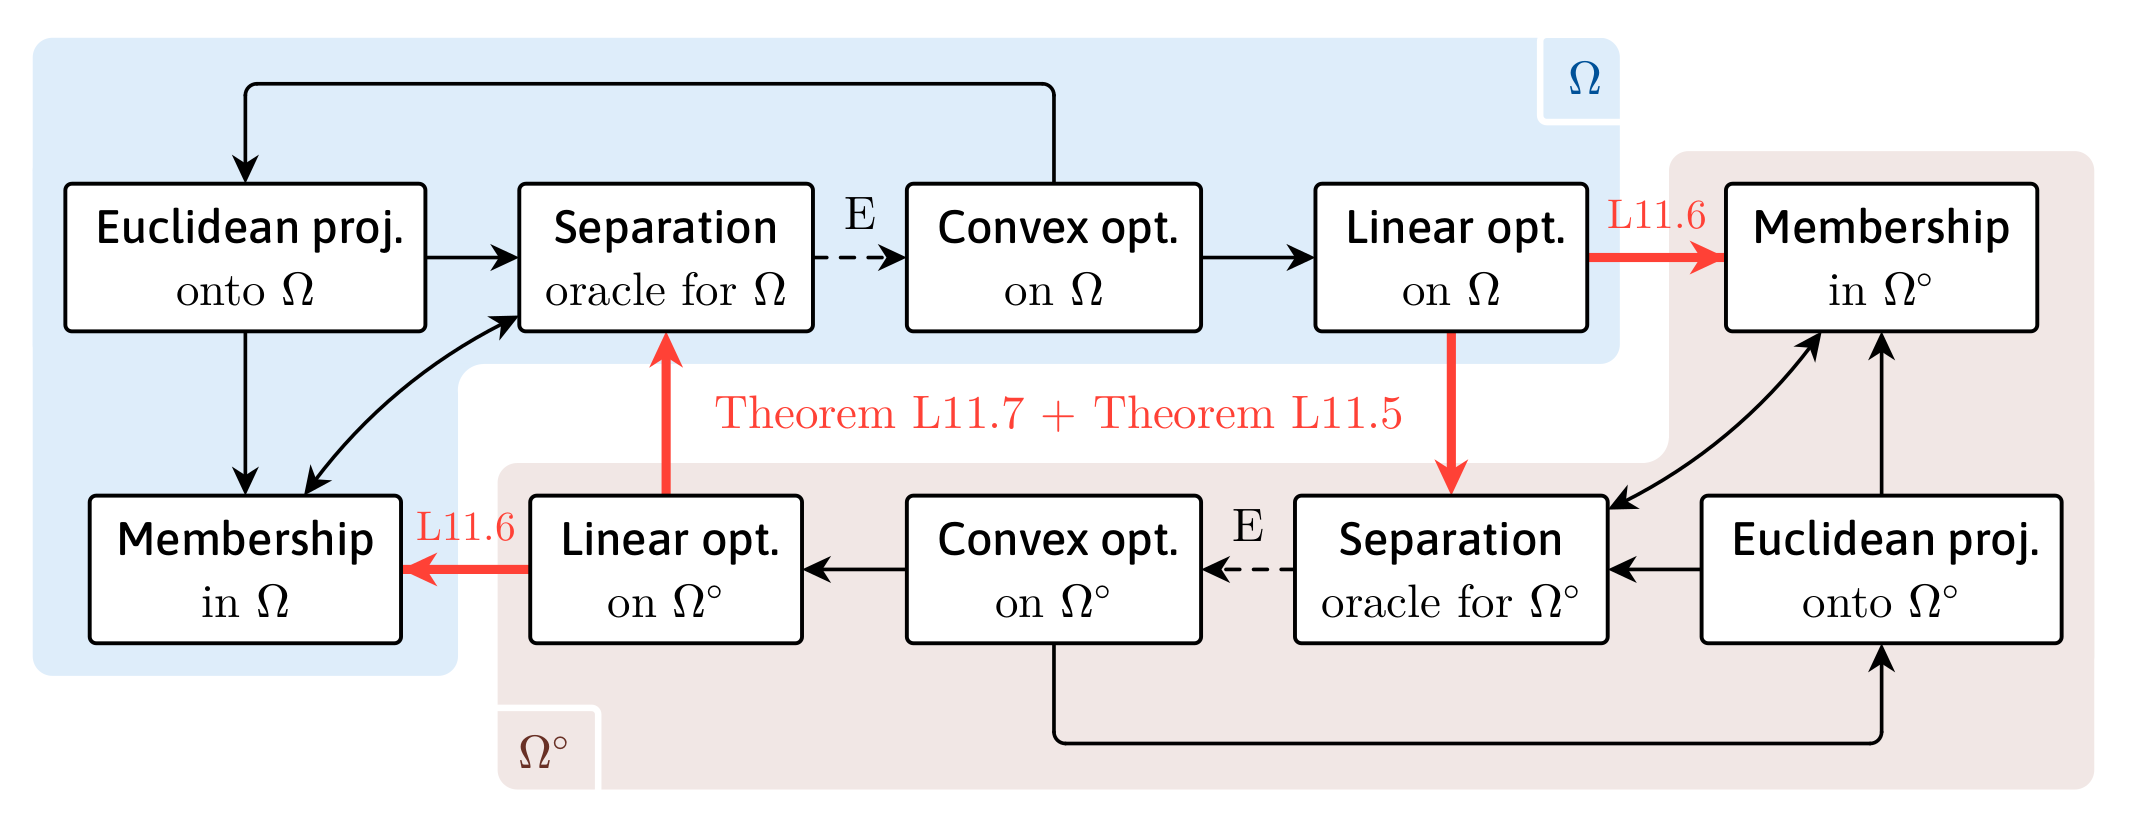
\includegraphics[width=\columnwidth]{figures/polarity.png}
\end{remark}

\begin{definition}[L11.1]{Polar set $\Omega^\circ$.}
    Let $\Omega$ be compact and convex, and such that $\mathbb{B}_r(0) \subseteq$ $\Omega \subseteq \mathbb{B}_R(0)$ for some radii $0<r \leq R$. The polar set $\Omega^{\circ}$ to $\Omega$ is defined as
    \vspace{-4pt}\\
    $$
    \Omega^{\circ}:=\left\{y \in \mathbb{R}^n:\langle x, y\rangle \leq 1 \quad \forall x \in \Omega\right\}
    $$
    \vspace{-4pt}
\end{definition}

\begin{theorem}[L11.5]{Involution of the polar set.}
    Theorem L11.5. Let the set $\Omega \subseteq \mathbb{R}^n$ be convex and compact, and such that $\mathbb{B}_r(0) \subseteq \Omega \subseteq$ $\mathbb{B}_R(0)$ for some $0<r \leq R$. Then,
    \begin{enumerate}[leftmargin=*]
        \item the polar set $\Omega^{\circ}$ is convex and compact, and satisfies $\mathbb{B}_{1 / R}(0) \subseteq \Omega^{\circ} \subseteq \mathbb{B}_{1 / r}(0)$; and
        \item the bipolar $\left(\Omega^{\circ}\right)^{\circ}$ is equal to $\Omega$.
    \end{enumerate}
\end{theorem}

\begin{theorem}[L11.6]{Polar membership oracle.}
    A membership oracle for $\Omega^{\circ}$ can be constructed efficiently starting from a linear optimization oracle for $\Omega$, even if the linear optimization oracle only returns the optimal objective value and not the minimizer.
    The construction only requires a single call to the linear optimization oracle.
\end{theorem}


\begin{theorem}[L11.7]{Separation oracle for the polar set.}
    A separation oracle for $\Omega^{\circ}$ can be constructed efficiently, without use of Section L11.2, starting from a linear optimization oracle for $\Omega$ that returns the optimal point.
    The construction only requires a single call to the linear optimization oracle.
\end{theorem}

\begin{remark}[X]{Additional notes:}
    with matrices, $Ax=b$ $\Leftrightarrow$ $\langle A_k,X \rangle = b_k$ $\forall k=1,...,m$. Where $\langle A_k,X \rangle = \text{tr}(AB^\top) = \sum_{i}\sum_{j}A_{ij}B_{ij}$.\\

    Nonnegative Cone $\rightarrow$ Linear Programs\\
    Lorentz Cone $\rightarrow$ Second Order Conic Programs\\

    Failure modes of constraint qualification: Primal has optimal solution, dual matches value of primal, yet dual does not have maximizer. Primal has optimal solution, dual has optimal solution, but values of problems differ.
\end{remark}